\documentclass[a4paper,12pt]{article}

\usepackage[latin1]{inputenc} % accents
\usepackage[T1]{fontenc}      % caract�res fran�ais
\usepackage{geometry}         % marges
\usepackage{lmodern}
\usepackage[french]{babel}
\usepackage{url,csquotes}
\usepackage[hidelinks,hyperfootnotes=false]{hyperref}
\usepackage{graphicx}
\usepackage[titlepage]{polytechnique}
%\usepackage{textcomp}
\usepackage{float}
\usepackage{enumerate}
\usepackage{enumitem}%textbullets
 \frenchbsetup{StandardLists=true}%textbullets
 \usepackage{soul}
 \usepackage{color}
 \usepackage{amsfonts}
 \usepackage{amsmath}
 \usepackage{tikz} %draw dots

\DeclareMathOperator{\e}{e}

\title{Low Dimensional Embedding of Environmental Variables}      % renseigne le titre
\subtitle{EA MAP581}
\author{Flore Martin and Lorraine Roulier}           %   "   "   l'auteur
%\date{\today}           %   "   "   la future date de parution
\renewcommand{\thesection}{\arabic{section}}

\definecolor{bleu}{rgb}{0.5, 1.0, 1.0}
\newcommand{\hlb}[1]{\sethlcolor{bleu}\hl{#1}}


\begin{document}

\maketitle
\tableofcontents
\newpage

\section{Introduction}

Climate data amounts very quickly to a lot of unused data. In a day, we can collect temperature, pressure, wind data all over the world with satellites, even hourly. Our project was two sided. First, we familiarized with various dimension reduction techniques, then we attempted to show that the geographical position of a point on the planet - e.g. it's latitude and longitude - were embedded in the climate data one could gather on it. 

Dimension reduction techniques can be divided in two classes, linear dimension reduction and non linear dimension reduction. However, in all methods, the main goal is to figure out a similarity function between vectors. Such a function will then enable to sort the dataset into classes of vectors with similar features, which would have been more intricate with the initial dataset. 
We used a set of datasets we found on the NASA website, that gathered various means on climate variables over 22 years at every given latitude and longitude. These variables are gathered in the table below

\begin{figure}[H]
 \begin{center}
	
	\begin{tabular}{|c|c|c|c|c|c|c|}
		 \hline    
	  	Latitude & Longitude &Temperature & Pressure&  Relative Humidity& Wind Speed& Radiation\\ 
		
		& & �$C$ & $kPa$ & $ \%$ & $m/s$ & $kWh/m^{2}/day$ \\ 
		\hline
		  \end{tabular}
\end{center}
\caption{Variables of our dataset}
\end{figure}

The latitude parameter varies from -90 to 89 and the longitude parameter varies from -180 to 179. the negative values are for the south hemisphere, the positive ones for the north. Depending on the running time of the method, we did not compute the dimension reduction with the 64800 lines, but with a subset. 
The subset is often a slice of longitudes containing all latitudes, as we assumed that the critical parameter to differenciate climate data was the latitude. 

\begin{figure}[H]
 \begin{center}
	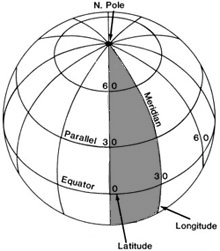
\includegraphics[scale = 4]{latlon.jpg}
\end{center}
\caption{An example of subset in grey}
\end{figure}

We classified the data according to the latitude, creating five classes listed in the table below. A more visual picture of our classification is given when we introduce the results of the different dimension reduction methods. 
\begin{figure}[H]
 \begin{center}
	
	\begin{tabular}{|c|c|c|c|c|c|}
		 \hline    
	  	& North &Temperate north & Equator &  Temperate South & South\\ 
		\hline
		Latitudes & 90 to 66 & 66 to 23 & 23 to -23 & -23 to -66 & -66 to -90 \\
		\hline
		 & \tikz\draw[blue,fill=blue] (0,0) circle (.5ex); & \tikz\draw[red,fill=red] (0,0) circle (.5ex); & \tikz\draw[green,fill=green] (0,0) circle (.5ex); & \tikz\draw[yellow,fill=yellow] (0,0) circle (.5ex); & \tikz\draw[pink,fill=pink] (0,0) circle (.5ex); \\
		\hline
		  \end{tabular}
\end{center}
\caption{Our classification  }
\end{figure}

\section{Principal Component Analysis - PCA}
	\subsection{Method}
	
		Principal Component Analysis detects tendencies in the data by maximizing the variance of the dataset matrix. 		
		Let $ X \in \mathbb{R}^{d \times n} $ be our dataset where d is the number of variables and n the sample size, PCA maximizes the following equation :
%%
\[ \| X - MM^{T}X \|^{2}_{F} \]
subject to $ M \in \mathcal{O}^{d \times r} $ where $ r<d $ and $ \mathcal{O}^{d \times r}  $ is the space of orthogonal matrix and we use the Froebenius norm.

The maximum of the previous function is reached by the covariance matrix of the dataset: the r greatest eigenvalues of $ XX^{T} = PDP^{T}$ yield the maximum $ M = P_{r} $ where the columns are the eigenvectors associated to the eigenvalues mentioned above. The largest eigenvalues point to the eigenvectors that contain the most information about the dataset. 

The new dataset is thus $ Y = P_{r}^{T}X $ of dimensions $ r \times n $. In this example, there are r principal components for the PCA. 
	\subsection{Results}
		\subsubsection{Two dimensions}
		
		We first implemented PCA and ran it with only two principal components, which yielded the following graph for the whole dataset. The associated eigenvectors were 
		\begin{align*}
			y_{1} &= \begin{bmatrix} 
					-0.94\\
					 -0.31 \\
					  0.11\\
					   -0.04\\
					     0.01
				      \end{bmatrix}
		\end{align*} 
		and 
		\begin{align*}
			y_{2} &= \begin{bmatrix} 
				      0.03\\
				       -0.40\\
				        -0.91 \\  
				        0.04\\
				         -0.05
				      \end{bmatrix}
		\end{align*} 
		
		This enables us to understand the meaning of these vectors. $ y_{1} $ is mostly related to a decreasing temperature and pressure, and $ y_{2} $ represents decreasing humidity and pressure. 

\begin{figure}[H]
	\centering
	\begin{minipage}[r]{.86\linewidth}
      		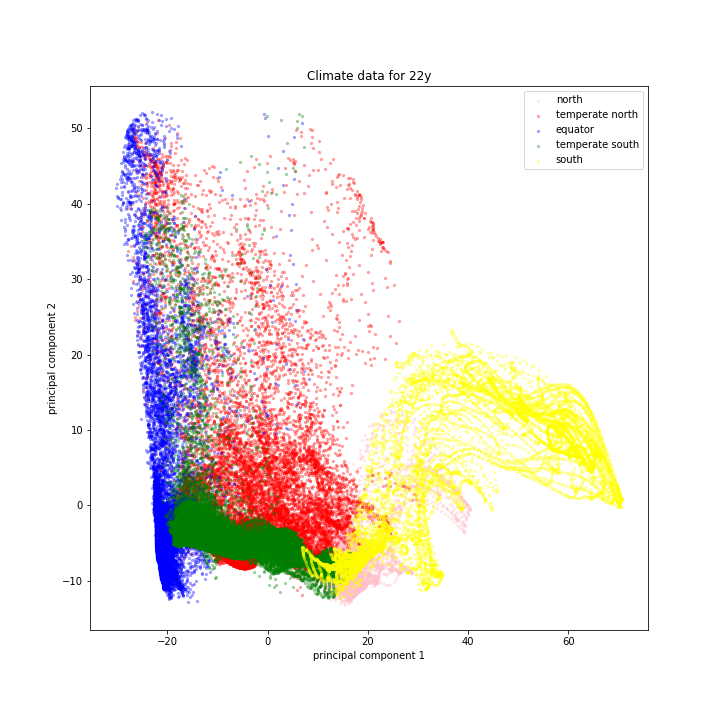
\includegraphics[scale=0.4]{pca2.png} %gauche bas droite haut
        \end{minipage}
         \hfill%
         \begin{minipage}[l]{.12\linewidth}
        		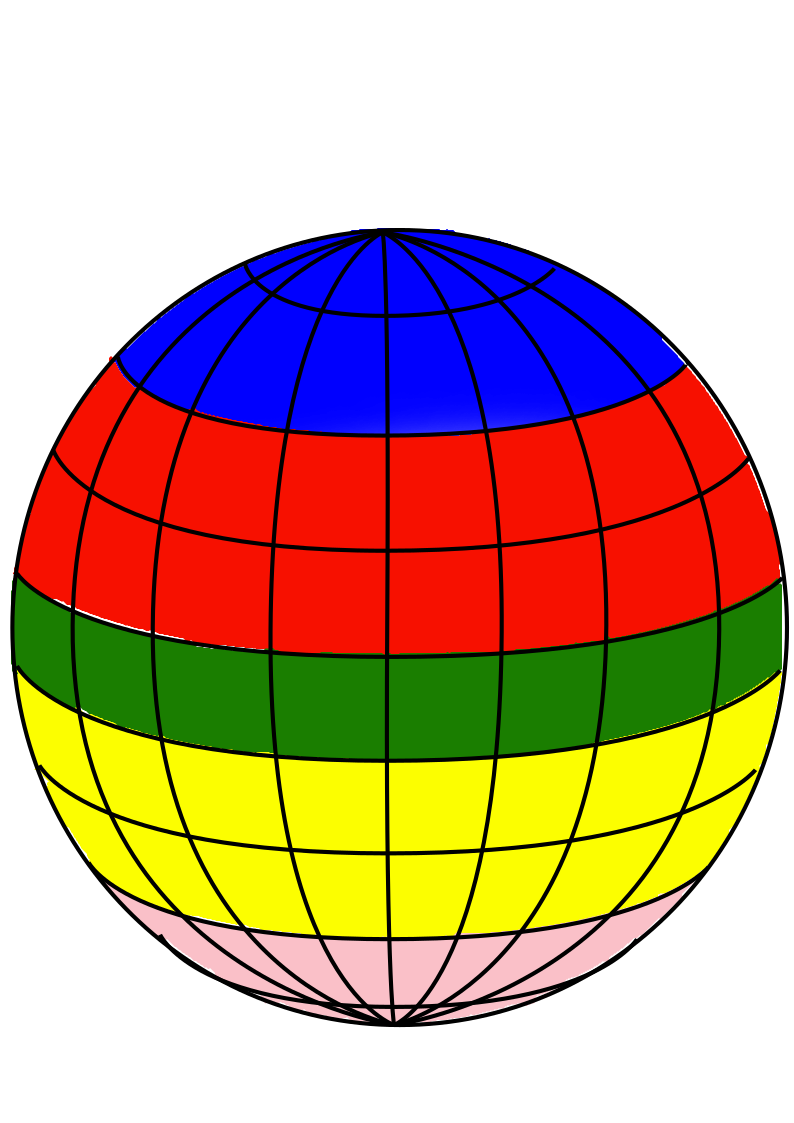
\includegraphics[scale=0.1]{colors.png}
    \end{minipage}
    \caption{PCA with two components}
\end{figure}

 \begin{center}
	\begin{tabular}{|c|c|c|c|c|}
		 \hline    
	  	 North &Temperate north & Equator &  Temperate South & South\\ 
		\hline
		  \tikz\draw[blue,fill=blue] (0,0) circle (.5ex); & \tikz\draw[red,fill=red] (0,0) circle (.5ex); & \tikz\draw[green,fill=green] (0,0) circle (.5ex); & \tikz\draw[yellow,fill=yellow] (0,0) circle (.5ex); & \tikz\draw[pink,fill=pink] (0,0) circle (.5ex); \\
		\hline
		  \end{tabular}
\end{center}

We can see on the graph that even if there is a strong dispersion, equator values are located at higher temperatures. On the contrary, north and south pole values are located at lower temperatures. Green and red classes overlap as these to categories have similar climate conditions. 

Although it is an understandable figure, this is not satisfying. We plot the eigenvalues to see their relative importance in the dimension reduction. 

\begin{figure}[H]
 \begin{center}
	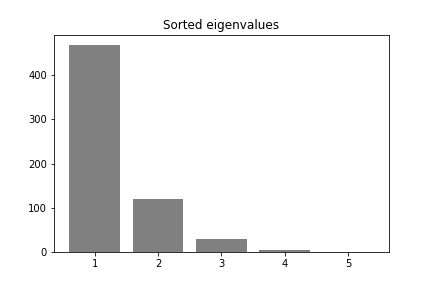
\includegraphics[scale = 0.6]{eigen.png}
\end{center}
\caption{PCA with two components}
\end{figure}

		\subsubsection{Three dimensions}
		
We attempted to run the PCA method with three principal components, 
		
		\subsubsection{Comparison of the dataset and its estimation by PCA}
		
		It is possible to built an estimated $ \hat{X} $ dataset from the projected data of PCA. We plotted the first column of the dataset, the temperature for $X $ and $ \hat{X} $ as a function of latitude and longitude. Even if the curve is reversed and the numerical values are not correct, the structure of the data is saved. 
		
\begin{figure}[H]
	\centering
	\begin{minipage}[c]{.30\linewidth}
       		 \centering
      		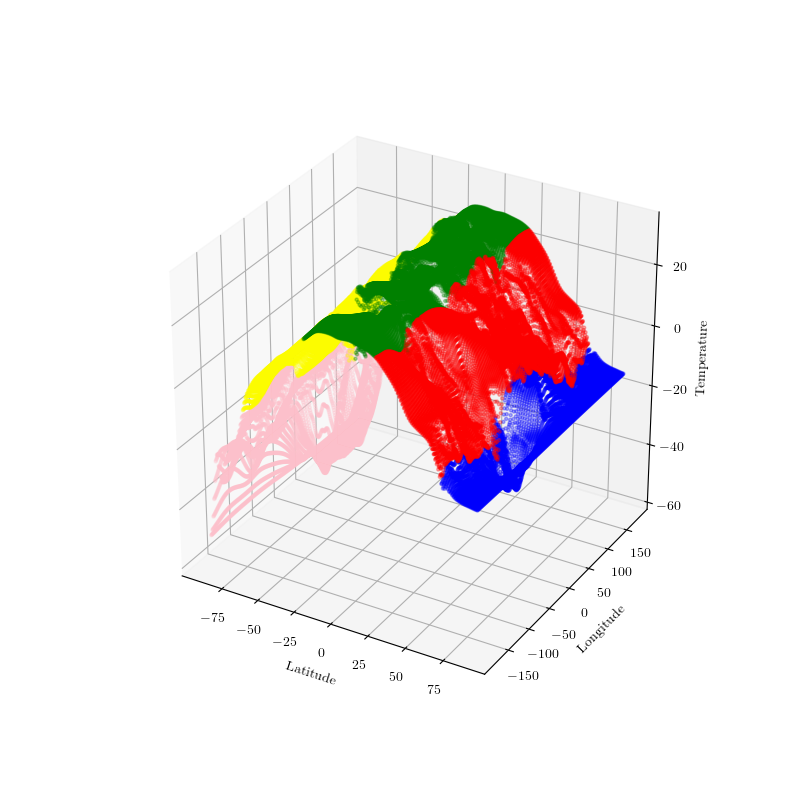
\includegraphics[scale=0.3]{temp1.png} %gauche bas droite haut
		\centering
        \end{minipage}
         \hfill%
         \begin{minipage}[c]{.30\linewidth}
                  \centering
        		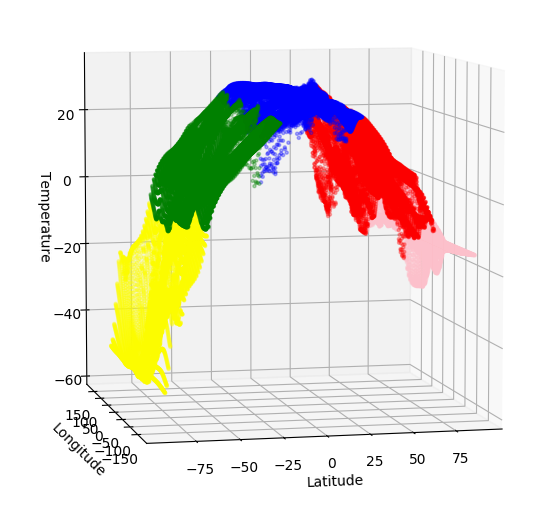
\includegraphics[scale=0.3]{temp2.png}
        		\centering
    \end{minipage}
     \begin{minipage}[c]{.30\linewidth}
                  \centering
        		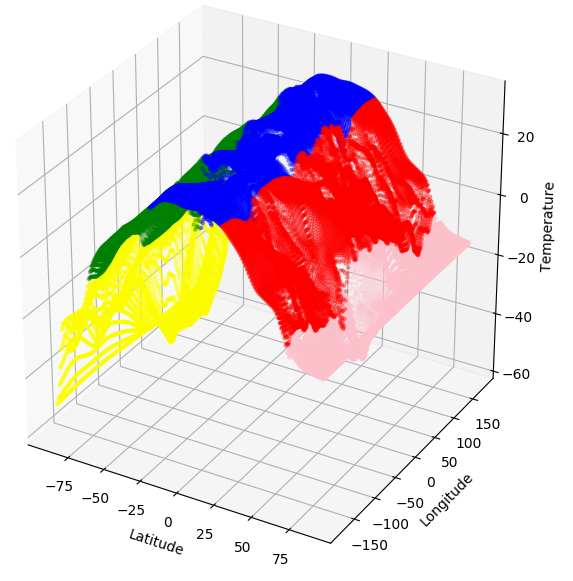
\includegraphics[scale=0.3]{temp3.png}
        		\centering
    \end{minipage}
    \caption{Temperature as a function of latitude and longitude in $X$ }
\end{figure}

\begin{figure}[H]
	\centering
	\begin{minipage}[c]{.30\linewidth}
       		 \centering
      		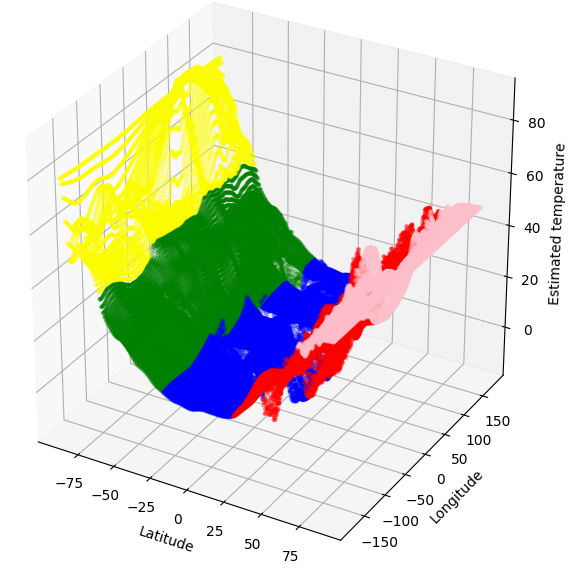
\includegraphics[scale=0.3]{esttemp1.png} %gauche bas droite haut
		\centering
        \end{minipage}
         \hfill%
         \begin{minipage}[c]{.30\linewidth}
                  \centering
        		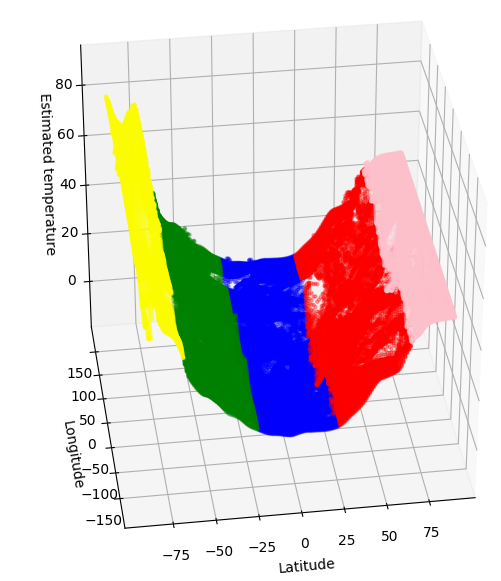
\includegraphics[scale=0.3]{esttemp2.png}
        		\centering
    \end{minipage}
     \begin{minipage}[c]{.30\linewidth}
                  \centering
        		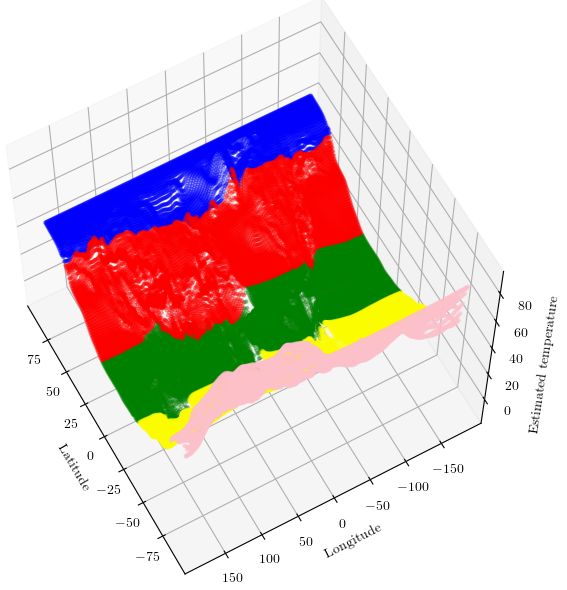
\includegraphics[scale=0.3]{esttemp3.png}
        		\centering
    \end{minipage}
    \caption{Temperature as a function of latitude and longitude in $\hat{X}$ }
\end{figure}


\section{Kernel Principal Component Analysis}
	\subsection{Method}
	
	Kernel Principal Component analysis is a non linear method for dimension reduction. Instead of directly maximizing the variance of $X$, we map it into a larger dimension space called the feature space, using a non linear function $\phi$. 
	
	Instead of directly mapping $X$ into the feature space, we use a kernel, that represents a similarity function between pairs. Let $K$ be this kernel, then 
	\[ K(x_{i},x_{j}) = \phi(x_{�}) \phi(x_{j})^{T}\]
where $x_{i}$�and $x_{j}$ are vectors of the dataset $X$ 
	
	This kernel will enable us to bypass the higher dimension calculation of the variance in the feature space. We only need to compute the pairwise values for $\phi$, but there is no need to explicitly define $\phi$.
	
	The downside of this method is that since we don't compute directly the eigenvectors and eigenvalues of $\phi$, the result is the projection of our dataset onto the eigenvectors. We thus don't have access to a simple interpretation of the principal components. 
	
	A classic kernel that is often used is the RBF function that is defined below: 
	 \[ K(x_{i},x_{j}) = \e{- \gamma \| x_{i} - x_{j} \| }\]

	\subsection{Results}
	
	Kernel PCA has a complexity of $ O(n^{3}) $ so we decided to run it on a subset of our dataset. Here is the two dimension result for all latitudes between longitudes -15 and +15. 
	
	
\begin{figure}[H]
 \begin{center}
	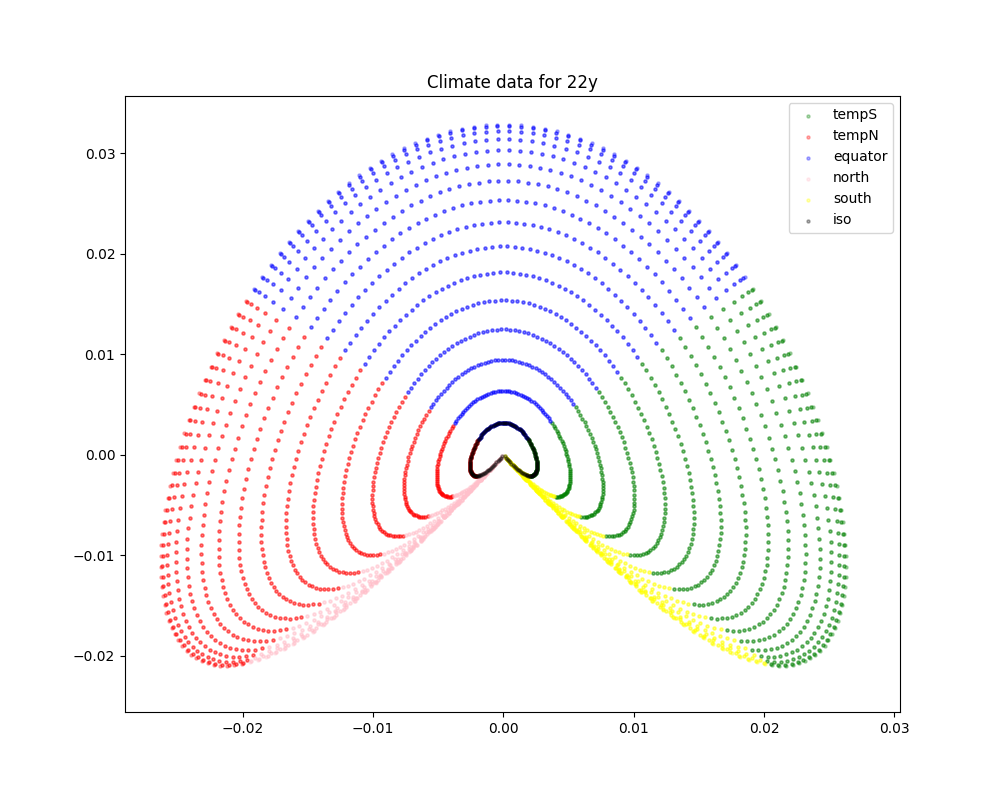
\includegraphics[scale = 0.5]{kpca_first.png}
\end{center}
\caption{Kernel PCA with two components and the RBF kernel}
\end{figure}

	The black dots are all dots along one longitude, here 15. We see however that there is a degenerescence: -15 and +15 longitude are projected on the same positions. When changing the gamma
	
	Another noticable flaw is the peak on the graph when we would expect the dots of same longitude to form a circle. The 3D visualisation of the graphic enables us to understand that peak: as we can see on the figure below, the lines that define one longitude form a sort of infinity symbol, a twisted circle, that can't render smoothly in two dimensions. 
	
\begin{figure}[H]
 \begin{center}
	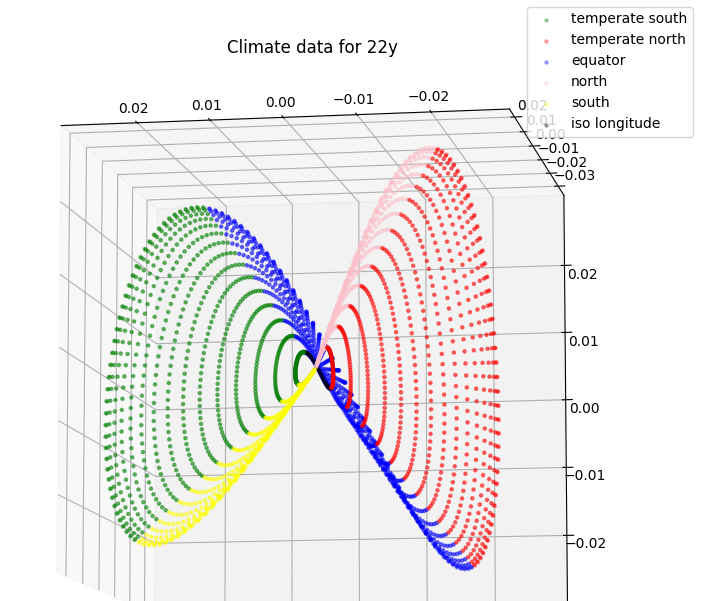
\includegraphics[scale = 0.5]{3Dkpca.png}
\end{center}
\caption{3D Kernel PCA}
\end{figure}

The dots representing the south and north poles are still closer together however, which might come from the smaller range of temperatures and climate conditions reached in these areas. 

We tried to change the $ \gamma $ parameter, but it had no influence on the degenerescence. Changing the kernel function to a polynomial one however destroyed the degenerescence, but created a node on equatorial values as it can be observed just below. The purple and black lines represent the -15 and 15 longitudes: they are clearly different. 

\begin{figure}[H]
 \begin{center}
	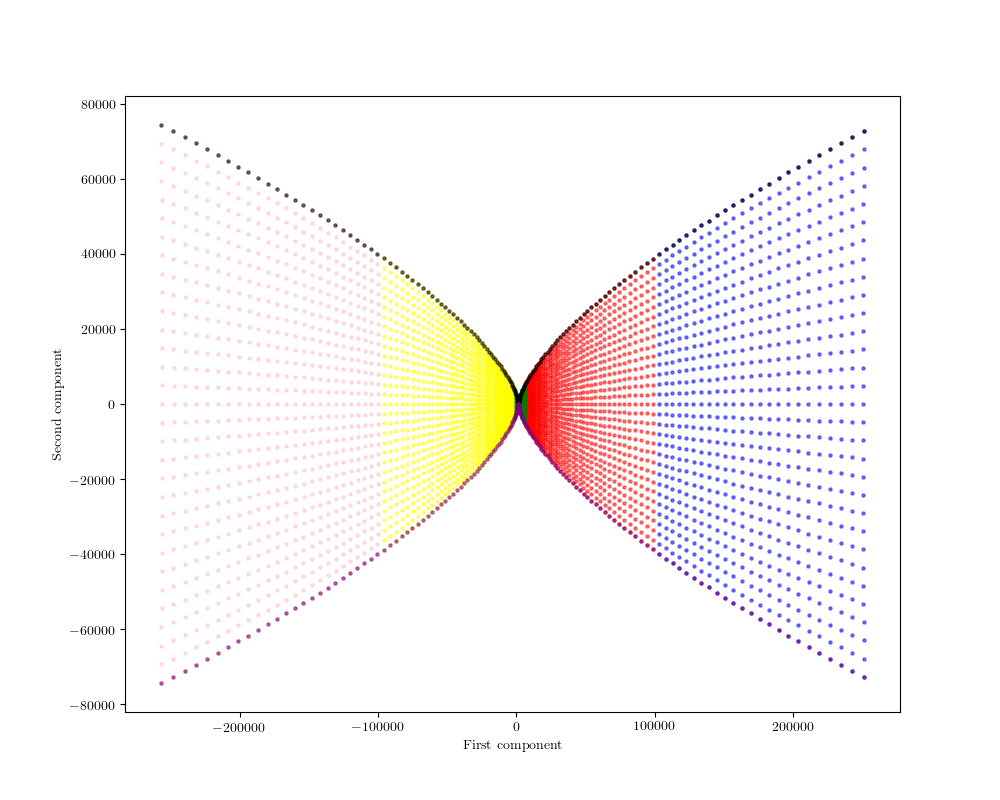
\includegraphics[scale = 0.5]{kpca_poly.png}
\end{center}
\caption{Kernel PCA with polynomial kernel}
\end{figure}


\section{Multidimensional Scaling - MDS}
	\subsection{Method}
	Multidimensional scaling is a non-linear approach to reduce dimension of a dataset. The principle is quite different from PCA: given a matrix of distance or "`dissimilarity"', MDS aims at reconstructing a map preserving at best the distances between datas. In our example, the MDS algorithm aims to place each object in 2-dimensional space such that the between-object distances are preserved as well as possible.
	Given a distance matrix D of dimension n*p (p=5 for us) , MDS attempts to find the datapoints $y_1$,... $y_t$ in dimension d<p (d=2 for us) that minimizes:
	
		 \[\sum\limits_{i=1}^{t}[\sum\limits_{j=1}^{t}d_{ij}^{(X)}-d_{ij}^{(Y)}]
			\]
		

	with $d_{ij}^{(X)}$ and $d_{ij}^{(Y)}$ respectively the euclidean distance between pairwise i and j in the original  n*p matrix $D^{(X)}$  and in the computed n*d matrix $D^{(Y)}$.
	
	As the distance matrix $D^{(X)}$  can be converted into a kernel matrix of inner products $X^TX$ by 
	\[ X^TX=-1/2HD^{(X)}H
		\]

H can be written as $H=I-ee^T$ and $e$ is the vector of ones. Thus, ??? becomes:
	\[\sum\limits_{i=1}^{t}\sum\limits_{j=1}^{t} x_{i}^{T}x_{j}-y_{i}^{T}y_{j}
		\]
	It can be shown that the solution is $Y=\Lambda^{1/2}V^T$ with $V$ the eigenvectors of $X^TX$ of the top d eigenvalues present in $\Lambda$.
	The only and main parameter of this method is the norm used to calculate the distance matrix. By default we use the euclidean norm here. 
	
	
	\subsection{Results}
	
	Figure 6 shows the results of MDS with our previous dataset. We use the same grandeurs (temperature, radiation, wind speed, humidity and pressure) but not the same number of lines. As MDS was extremeley low and seemed to use a lot of memory, we could not run the programm for more than 600 rows. Here are the result for 546 rows: we filtered our dataset with latitudes < 0 (ie. south hemisphere) and longitude between 0 and 5 degrees. 
	
	\begin{figure}[H]
 \begin{center}
	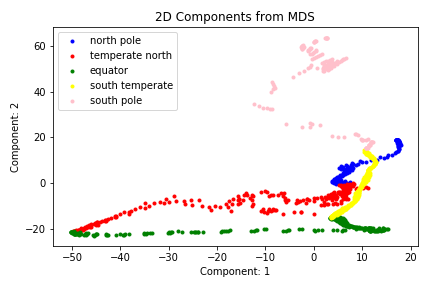
\includegraphics[scale = 1]{graphMDS.png}
\end{center}
\caption{results of MDS in 2D}
\end{figure}
	
	One indicator to estimate of the reconstruction is accurate is the 'stress'. It is roughly the square difference between the final distance of two items in the MDS model and the true distance between them. The exact formula is: 
		
			\[ s = \sqrt{\frac{\sum (d_{ij}-d(i,j))}{\sum d_{ij}}}
		\]
		
		The aim of MDS is to minimize this stress. Figure 7 presents the value of stress depending on the number of lines. We can see it is relatively low (<0,002) for more than 500 rows.
		
	\begin{figure}[H]
 \begin{center}
	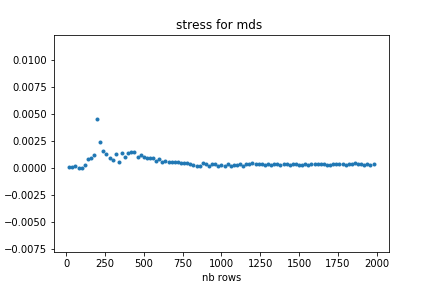
\includegraphics[scale = 1]{stressMDSnblines.png}
\end{center}
\caption{stress as a function of number of rows}
\end{figure}

\section{Isomap}
	\subsection{Method}
	
	Isomap is a low dimensional embedding method similar to MDS. The difference is, distance is not computed with euclidean norm but with geodesic distance. 
	\subsection{Results}
	
	As the main parameter of the method is the number of nearest neighbors taken into account, we present infigure 8 the result of isomap for number of neighbour from 1 to 11 neighbors. 
	
	\begin{figure}[H]
 \begin{center}
	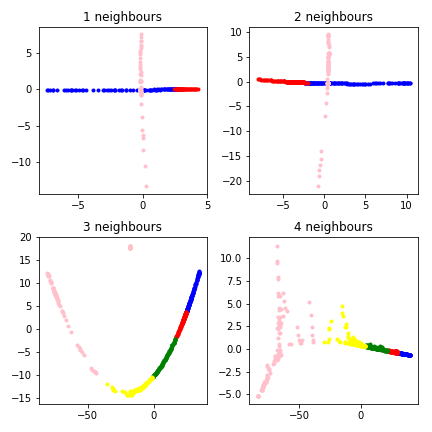
\includegraphics[scale = 0.5]{graphiso.png}
\end{center}
\caption{results of isomap depending on the number of neighbors considered from 2 to 12}
\end{figure}

It is obvious that the number of neighbours considered strongly influence the 2D distribution of our dataset. To know which graph is the most accurate, we refer to the 'reconstruction error'. We computed this reconsruction error with respect to the number of neighbours considered. The results are presented in figure ??

We also computed the error reconstruction as a function of the number of rows in figure 9. This error keeps increasing with the number or rows, so isomap accuracy seems to be limited by the size of the dataset.

\begin{figure}[H]
 \begin{center}
	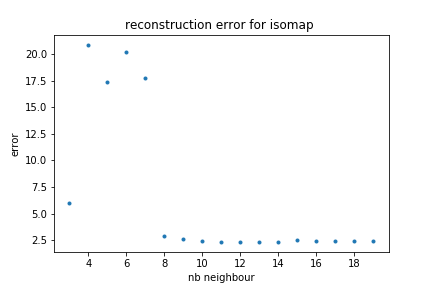
\includegraphics[scale = 0.8]{isoerrorneighbour.png}
\end{center}
\caption{reconstruction error as a function of number of neighbours considered}
\end{figure}

It is interesting to see that from eight neighbours, error seems to stabilize around 2,5. Indeed, we can see with graphs of figure 8 that from eight neighbours, graphs look quite all the same. Those are the most 'accurate' representations.
	
\section{Comparing the different methods}

	\subsection{Time comparison}
	
	We implemented manually PCA, but for the other methods we used the built in fonction of the scikit package on python. 
	PCA's running time varies linearly with the number of rows as we can see on the graphic below 

\begin{figure}[H]
 \begin{center}
	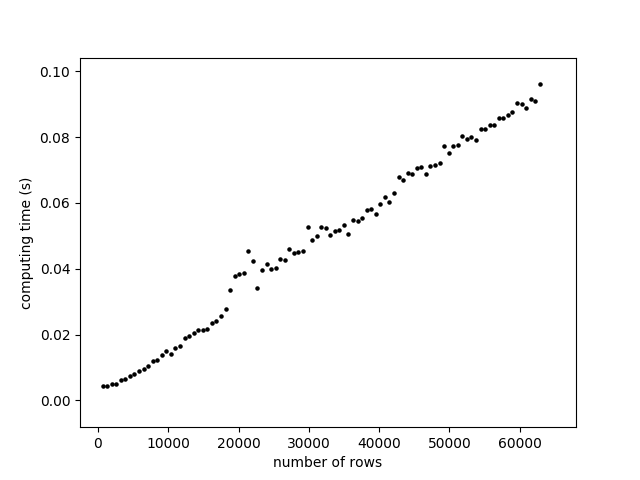
\includegraphics[scale = 0.8]{pcatime.png}
\end{center}
\caption{running time for PCA}
\end{figure}

Kernel PCA was slower, we did not compute its running time for all the dataset, only until 12000 rows. It yields the following graph. 

\begin{figure}[H]
	\centering
	\begin{minipage}[c]{.46\linewidth}
       		 \centering
      		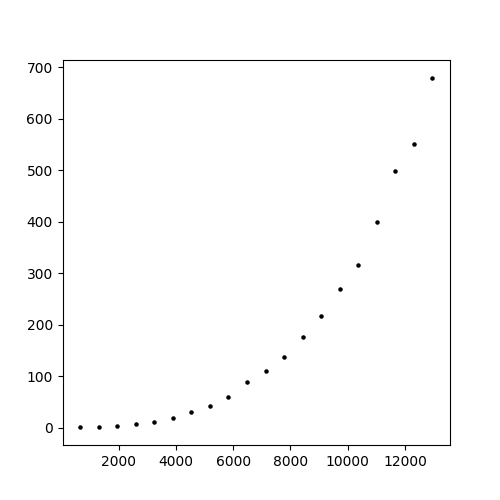
\includegraphics[scale=0.5]{kpcatime.png} %gauche bas droite haut
		\centering
		\caption{running time for Kernel PCA}
        \end{minipage}
         \hfill%
         \begin{minipage}[c]{.46\linewidth}
                  \centering
        		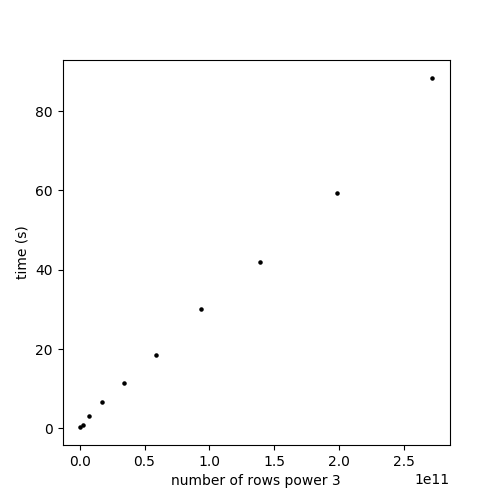
\includegraphics[scale=0.5]{kpcatimpe.png}
        		\centering
		\caption{Kernel PCA running time is a $O(n^{3})$}
    \end{minipage}
\end{figure}

	In figure 10, we present computing time for different methods as a function of the number of rows.
	From this we can conclude that the quickest method is PCA. Then comes kernel PCA, isomap and MDS. It is quite surprising to see that isomap is quicker than MDS for the same number of rows. Indeed, isomap uses the same algorithm than MDS but also needs to compute distance with neighbors first. It is thus expected to be slower. We found an explanation on the "`manifold guide"' of skicit.
	
	\begin{quotation}
\begin{quote}
In Scikit-Learn implementation, Isomap algorithm runs faster that Multi Dimensional Scaling on the S-Curve dataset [...]. In the third stage of algorithm, the implementation uses Partial Eigen Value decomposition instead of MDS which is the version proposed by the researchers	
	\end{quote}		
	\end{quotation}
	
	We did not use the "`S curve dataset"' as mentioned above, but we may think that due to the round shape of earth, our dataset is quite similar to the S-curve and thus Isomap runs faster than MDS.
	
	
	
		\begin{tabular}{|c|c|c|c|c|}
		 \hline    
	  	Method & PCA & Kernel PCA & MDS & Isomap \\ 
		\hline
		Complexity & $O(n)$ & $O(n^3)$ & $O(n^3)$  &  \\
		\hline
		  \end{tabular}
	

	
\begin{figure}[H]
 \begin{center}
	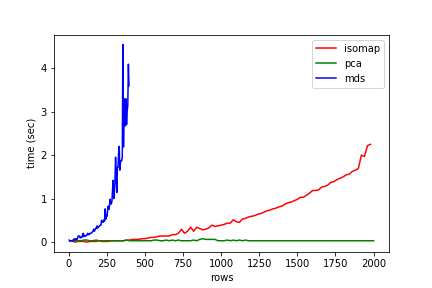
\includegraphics[scale = 0.8]{isomdstime.png}
\end{center}
\caption{computing time comparison}
\end{figure}


We also check how isomap computing time varies with the number of neighbor taken into account. Figure 11 shows that isomap efficiency time increases with the number of neighbors. So isomap efficiency of computing time may be limited by the number of neighbors.
\begin{figure}[H]
 \begin{center}
	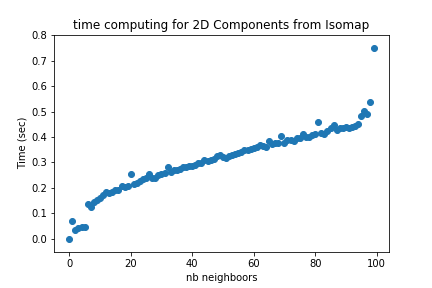
\includegraphics[scale = 0.8]{timeisoneigh.png}
\end{center}
\caption{computing time for isomap as a function of the number of neighbors considered}
\end{figure}

\subsection{Error and preserved information}

\section{Conclusion}
\section{Bibliography}


\end{document}
